\documentclass[12pt]{article}
\usepackage[utf8]{inputenc}
\usepackage[usenames]{color}
\usepackage[margin=1in]{geometry} 
\usepackage{amsmath,amsthm,amssymb,graphicx,mathtools,tikz,hyperref, pgfplots, listings, pdfpages}
\usetikzlibrary{positioning}
\newcommand{\n}{\mathbb{N}}
\newcommand{\z}{\mathbb{Z}}
\newcommand{\q}{\mathbb{Q}}
\newcommand{\cx}{\mathbb{C}}
\newcommand{\real}{\mathbb{R}}
\newcommand{\field}{\mathbb{F}}
\newcommand{\ita}[1]{\textit{#1}}
\newcommand{\com}[2]{#1\backslash#2}
\newcommand{\oneton}{\{1,2,3,...,n\}}
\newcommand\idea[1]{\begin{gather*}#1\end{gather*}}
\newcommand\ef{\ita{f} }
\newcommand\eff{\ita{f}}
\newcommand\proofs[1]{\begin{proof}#1\end{proof}}
\newcommand\inv[1]{#1^{-1}}
\newcommand\setb[1]{\{#1\}}
\newcommand\en{\ita{n }}
\newcommand{\vbrack}[1]{\langle #1\rangle}


\newenvironment{theorem}[2][Teorema]{\begin{trivlist}
\item[\hskip \labelsep {\bfseries #1}\hskip \labelsep {\bfseries #2.}]}{\end{trivlist}}
\newenvironment{lemma}[2][Lema]{\begin{trivlist}
\item[\hskip \labelsep {\bfseries #1}\hskip \labelsep {\bfseries #2.}]}{\end{trivlist}}
\newenvironment{exercise}[2][Ejercicio]{\begin{trivlist}
\item[\hskip \labelsep {\bfseries #1}\hskip \labelsep {\bfseries #2.}]}{\end{trivlist}}
\newenvironment{reflection}[2][Reflexión]{\begin{trivlist}
\item[\hskip \labelsep {\bfseries #1}\hskip \labelsep {\bfseries #2.}]}{\end{trivlist}}
\newenvironment{proposition}[2][Proposición]{\begin{trivlist}
\item[\hskip \labelsep {\bfseries #1}\hskip \labelsep {\bfseries #2.}]}{\end{trivlist}}
\newenvironment{corollary}[2][Corolario]{\begin{trivlist}
\item[\hskip \labelsep {\bfseries #1}\hskip \labelsep {\bfseries #2.}]}{\end{trivlist}}
 \hypersetup{
 colorlinks,
 linkcolor=blue
 }

\renewcommand{\ttdefault}{pcr}
\lstdefinestyle{C}{language=C,
    basicstyle=\ttfamily,
    keywordstyle=\bfseries,
    showstringspaces=false,
    morekeywords={include, printf},
	keepspaces=true,numbers=left,xleftmargin=2em,frame=shadowbox,framexleftmargin=0 em, rulesepcolor = \color{black}
}
\lstdefinestyle{linuxterminal}{language=bash,
    basicstyle=\ttfamily,
    keywordstyle=\bfseries,
    showstringspaces=false,
    morekeywords={include, printf},
	keepspaces=true,
	frame=TLRB
}


\begin{document}
	\date{04-03-2018}
	
	
	\title{\textbf{\textcolor{red}{INFORME PRÁCTICA 1}}}
	\author{Alejandro Santorum Varela - alejandro.santorum@estudiante.uam.es\\David Cabornero Pascual - david.cabornero@estudiante.uam.es\\Pareja 7\\Universidad Autónoma de Madrid}
	\maketitle
	
	\tableofcontents
	
	\newpage
	
	
\section{Introducción}
Ese documento recoge los ejercicios realizados en la primera práctica de Sistemas Operativos.\\\\
Para cada ejercicio se comentará su diseño, su funcionalidad detalla y un análisis de las diferentes decisiones tomadas a la hora de enfrentarse a los problemas o dificultades encontradas. Anteriormente se incluia el código, pero en esta versión final se ha prescindido del mismo ya que se puede acceder a el en la carpeta de la entrega.\\


\section{Ejercicio 4-A}
Empezamos con el primero ejercicio entregable de la práctica, el ejercicio 4a. Se pedía examinar el código aportado y modificarlo tal que cada hijo imprima su PID y el PID de su proceso padre.\\\\
Se ha modificado el código tal que ahora el hijo es el que imprime los PID's en lugar de que cada uno imprima el suyo. También se ha introducido una nueva comprobación para saber si el proceso ha quedado huérfano, cosa que se especifica al final del enunciado del ejercicio 4b.\\\\
Se muestra ahora la salida de este programa en Linux:
\begin{center}
	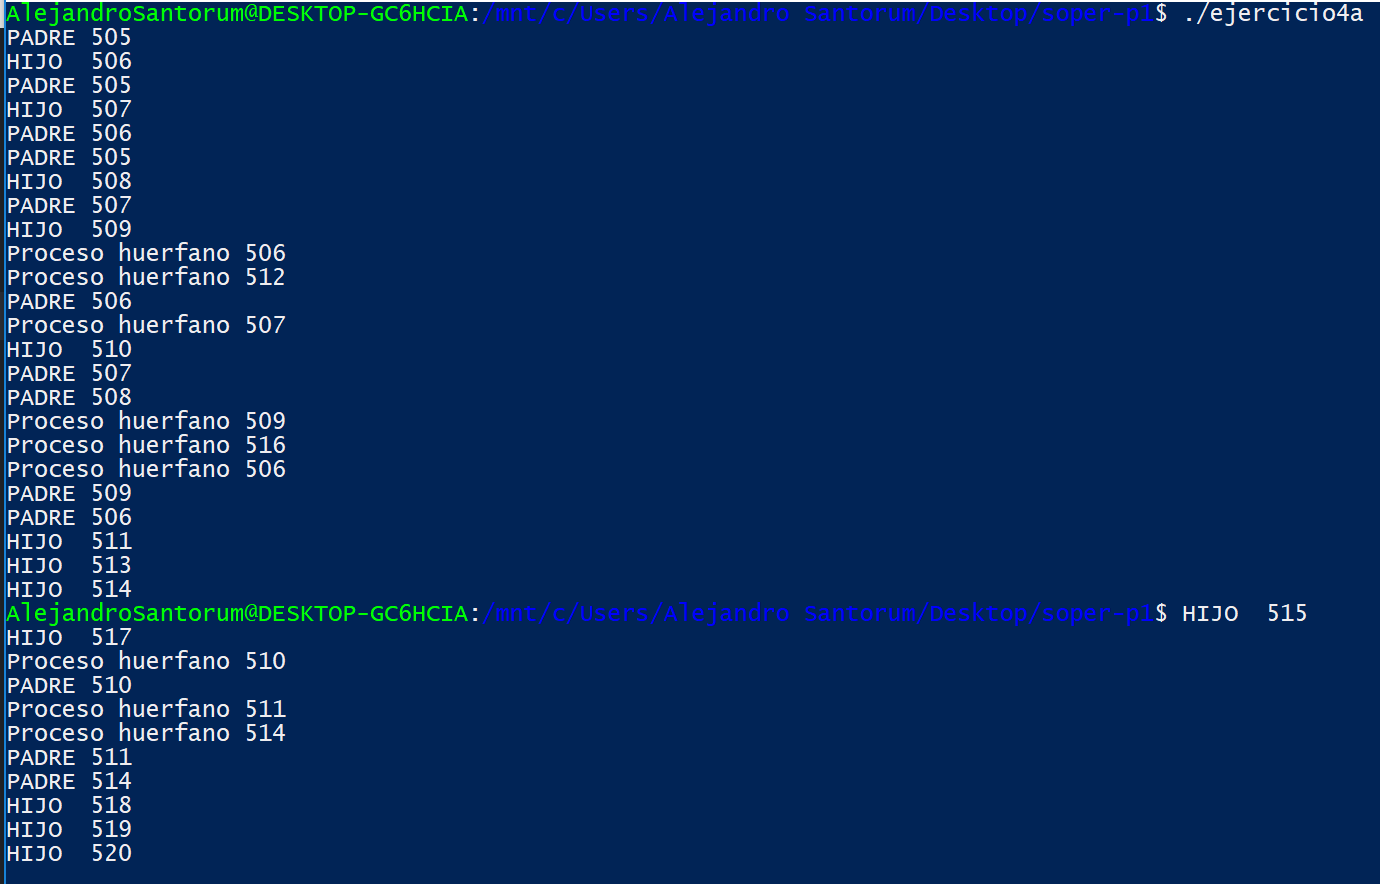
\includegraphics[scale=0.9]{ej4a.PNG}
\end{center}
Se comentará esta salida junto con la salida del ejercicio 4b más adelante.\\


\section{Ejercicio 4-B}
El ejercicio 4b es una extensión del 4a, con la única modificación de incluir un wait() al final del programa.\\\\
Igual que en el ejercicio 4a, se pedía que cada hijo imprimise su PID y el de su proceso padre, de ahí que los cambios sean idénticos. También se preguntaba por la funcionalidad de wait(), lo cual se comentará después de observar la salida de este programa.
\begin{center}
	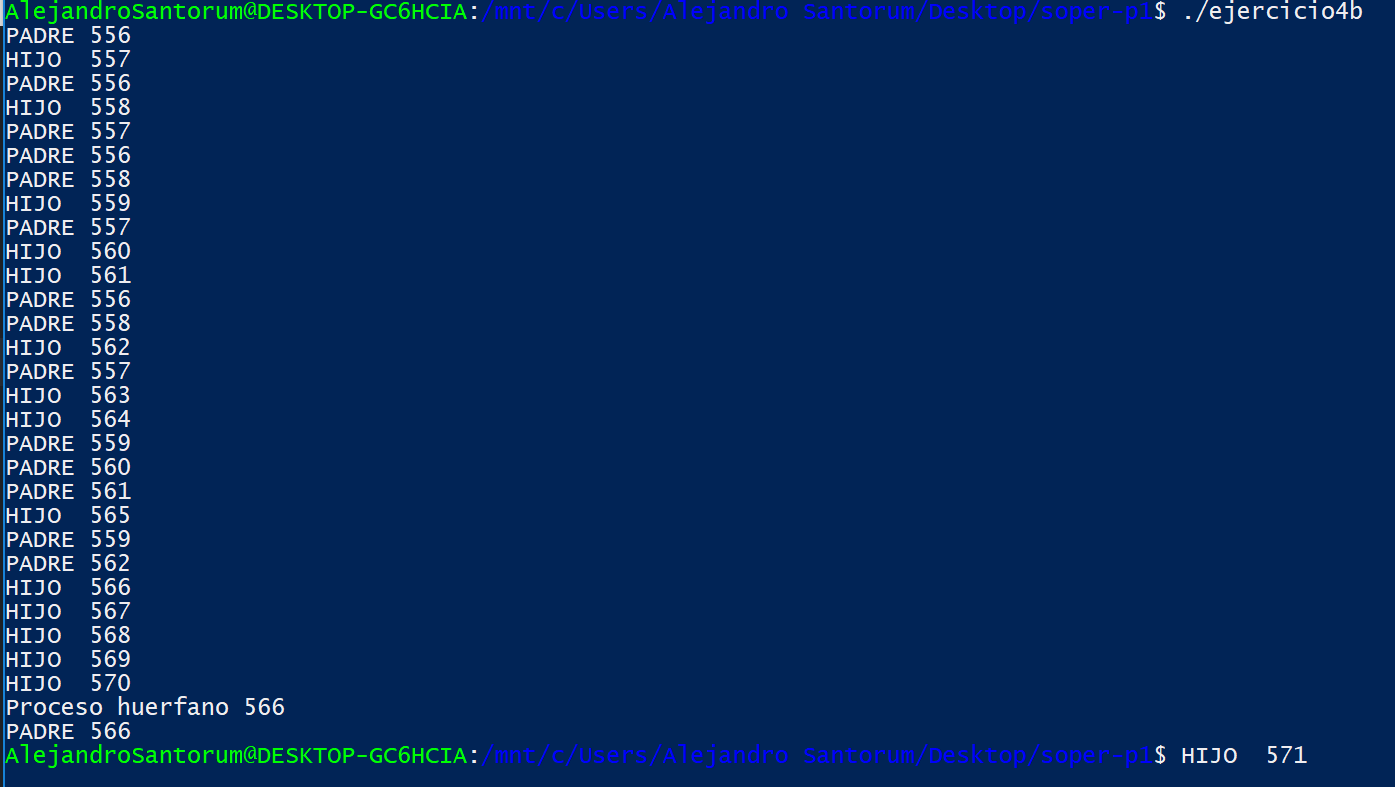
\includegraphics[scale=0.9]{ej4b.PNG}
\end{center}
En este momento ya tenemos ejemplos suficientes, con la salida del 4a y del 4b, para comentar sus diferencias y el objetivo del wait().\\\\
Por un lado, lo primero que salta a los ojos es la diferencia de procesos huérfanos que genera. Esto es debido a que la función wait() en un proceso lo obliga a esperar a que \textbf{alguno} de sus procesos hijos (si los tiene) acabe su ejecución, por lo que la cantidad de procesos huérfanos es reducida, ya que es más complicado que algún proceso acabe después que su padre porque este tiene pocos hijos (en este programa) y espera por alguno.\\\\
Por otro lado, también se puede observar que el prompt de la terminal se realiza prácticamente después de finalizar la ejecución de todos los procesos (menos uno en este caso), a diferencia que el ejercicio 4a que saltaba cuando aún no habían finalizado aproximadamente un cuarto de los procesos.\\\\
Por último, se recomienda utilizar el comando pstree -p para percibir el árbol de procesos que se origina. Aquí un ejemplo.
\begin{center}
	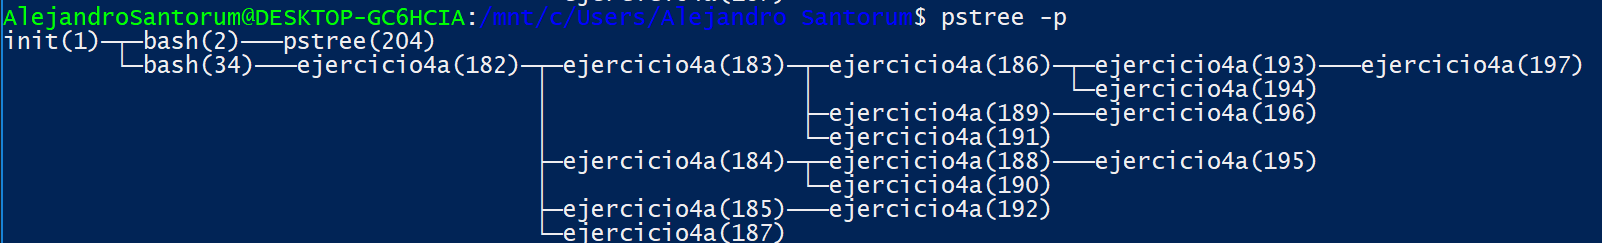
\includegraphics[scale=0.78]{ej4_pstree.PNG}
\end{center}
Desafortunadamente no se puede obtener una buena panorámica de la diferencia de construcción-desaparición de procesos en el árbol entre los ejercicios 4a y 4b. De todas formas, podemos predicir como va evolucionando. El proceso de construcción del árbol es idéntico en ambos casos (hasta un resultado final como el de la imagen); es en el transcurso de desaparición de nodos en el árbol en lo que varian los programas: en el primero, si pudiésemos ejecutar pstree cada vez que acaba un proceso, podríamos ver como muchos acaban sin proceso padre y son "adoptados" por el proceso de PID=1, init. En el segundo, podríamos ver que los procesos van desapareciendo prácticamente en orden, los padres después de alguno de sus hijos.\\


\section{Ejercicio 5-A}
En el ejercicio 5a se nos pide realizar los mínimos cambios posibles en el programa del ejercicio 4b de forma que se generen un conjunto de procesos hijos secuencial de modo que cada proceso tiene un único proceso hijo y ha de esperar a que finalice.\\\\
El programa se ha modificado únicamente en la línea 23(sin contar el cambio de i\%2==0 por i\%2!=0 que especifica el enunciado), la sentencia \texttt{else break;} realiza la importante misión de que si el proceso no tiene la variable pid==0 quiere decir que está corriendo como padre, y por lo tanto no puede hacer más forks. Una forma muy buena de ver como se van originando los procesos es utilizar la función pstree -p enseñada en el ejercicio anterior.
\begin{center}
	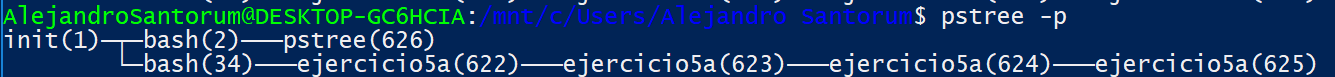
\includegraphics[scale=0.95]{ej5a_pstree.PNG}
\end{center}
No hay duda de que cada proceso crea uno hijo y solo uno.\\\\
Además, se establecía que cada proceso tenía que esperar por la finalización de su hijo para acabar, lo cual es percibe bastante bien en la salida del programa.
\begin{center}
	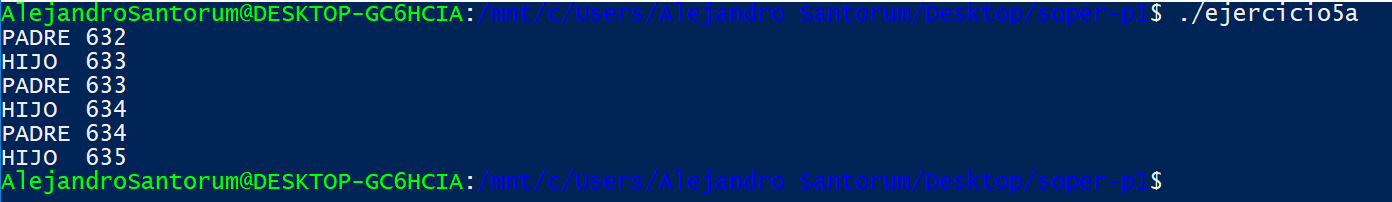
\includegraphics[scale=0.9]{ej5a.PNG}
\end{center}
A diferencia que en los ejercicios 4a y 4b, los PID's se imprimen en la terminal por orden, siempre en parejas PADRE-HIJO. En el ejercicio anterior esto no pasaba porque todos los programas estaban ejecutándose al mismo tiempo, haciendo que mientras uno imprimía PADRE-HIJO, otro proceso hacía lo mismo, dando un resultado en la terminal de, por ejemplo, PADRE PADRE HIJO HIJO.\\


\section{Ejercicio 5-B}
En el ejercicio 5b, como en el 5a, se nos pide realizar los mínimos cambios posibles en el programa del ejercicio 4b, pero ahora un único proceso padre origina un conjunto de procesos hijos y este ha de esperar a que acaben todos los procesos hijos antes de finalizar.\\\\
La clave de este ejercicio está en darse de cuenta que si la variable pid es igual a cero (en el momento que imprime su PID y el de su padre), es que está funcionando en ese momento como un proceso hijo, por lo que no puede hacer más forks, de ahí la sentencia \texttt{break;}.\\\\
Otro elemento de gran peso en el programa es en la línea 28 la instrucción \texttt{while(wait(NULL)>=0);}, que es la encargada de que el proceso padre espere por \textbf{todos} sus procesos hijos a que finalicen. Esto es así porque wait() devuelve un número negativo cuando no tiene hijos ejecutándose, por lo que el while realiza la función de esperar a que todos hayan termiando.\\\\
A continuación se muestra la salida por la terminal y el árbol generado.
\begin{center}
	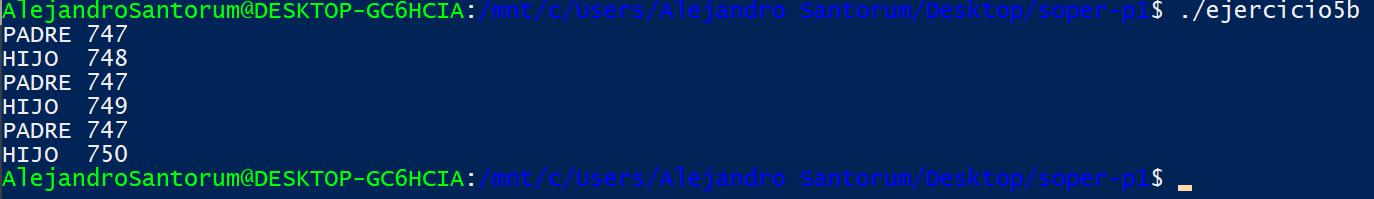
\includegraphics[scale=0.85]{ej5b.PNG}
\end{center}
\begin{center}
	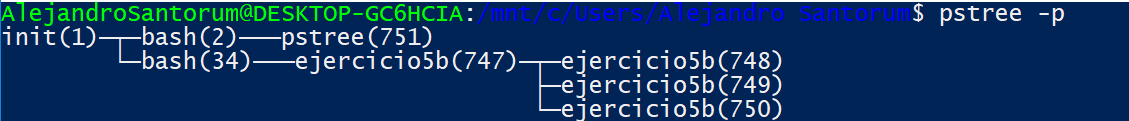
\includegraphics[scale=1.03]{ej5b_pstree.PNG}
\end{center}
En el árbol se puede ver perfectamente que un padre origina un conjunto de procesos hijos. Además, en la salida de la terminal podemos ver que el PID del padre es siempre el mismo.\\


\section{Ejercicio 6}
Este ejercicio tiene la misión de enseñar como funciona la memoria dinámica con procesos de por medio. El ejercicio pedía que el proceso padre reservase memoria dinámica para una estructura que albergase una cadena de 80 caracteres y un entero. A continuación debía generar un proceso hijo y que este pidiese al usuario un nombre para guardar en la estructura, para luego comprobar si el proceso padre tenía acceso a esa cadena guardada en el hijo.\\\\
El código en el fichero fuente se encuentra comentado a diferencia del mostrado aquí.\\El principio del programa es trivial, declaración de la estructura y reserva de memoria para la misma. A continuación se guarda en la cadena el texto "TEXTO GUARDADO ANTES DEL FORK" para poder ver que se imprime en el proceso padre después de que en el hijo se haya sobreescrito la cadena con el nombre itroducido.\\\\
Como era de esperar, se realiza el fork, si pid==0 estamos en el proceso hijo y por lo tanto pedimos al usuario un nombre, el cual guardamos en la cadena de la estructura. Una ves de vuelta en el proceso padre (especial atención al wait() para esperar al proceso hijo) se imprime el contenido de la cadena por pantalla.\\\\
Se muestra ahora la salida del programa.
\begin{center}
	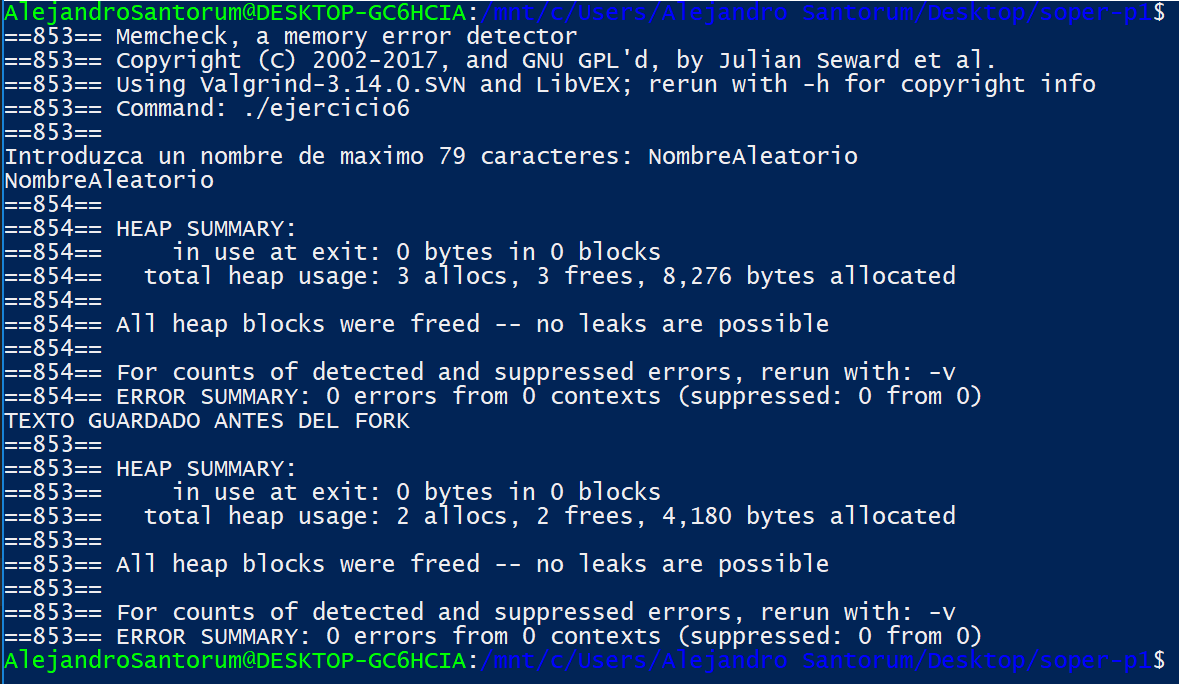
\includegraphics[scale=1]{ej6.PNG}
\end{center}
Esto contesta a varias de las preguntas. Se puede inferir que las modificaciones adoptadas en el proceso hijo en la cadana no interfiere en la cadena del proceso padre, por lo que se puede deducir que al hacer un fork la memoria reservada es duplicada, una zona de memoria contendrá las variables del proceso padre y otra zona para los datos del hijo. Después del wait(), cada uno imprime su contenido, dando como resultado que la estructura del padre no ha recibido modificaciones y la del hijo tiene la cadena introducida por pantalla.\\\\
Por último, en el programa se ha liberado la memoria reservada en ambos procesos debido a que, como se ha dicho, cuando se hace fork se duplica la memoria reservada y cada proceso continua accediendo a la suya. Se adjunta en la imagen el reporte de memoria de Valgrind, el cual ratifica lo dicho anteriormente.\\


\section{Ejercicio 8}
Este es uno de los ejercicios más complejos y enriquecedores de la práctica en nuestra opinión. Junto los forks y waits con una nueva familia de funciones desconocida para nosotros; y este ejercicio nos ha ayudado en gran medida a comprender su utilidad y funcionamiento.\\\\
Se nos pide escribir un programa que cree tantos procesos hijos como programas ejecutables reciba el proceso padre como argumentos de entrada. Además, dependiendo del último argumento de entrada, se llamará a la ejecución de estos programas usando cuatro funciones diferentes de la familia exec() descritas en la documentación de la práctica.\\\\
A pesar de que se especifica en el enunciado que el orden de ejecución es desde el primero al último, hemos hecho otro segundo programa casi idéntico al primero que en lugar de ejecutar desde el principio hasta el programa $n$, empieza ejecutando el programa $n$-ésimo hasta el primero pasado como argumento de entrada. Son respectivamente, los programas denominados como \texttt{ejercicio8\_1.c} y \texttt{ejercicio8\_2-c}. \\\\
Se puede resumir la funcionalidad del código de la siguiente forma. Primero, se comprueban los parámetros de entrada del programa principal buscando que no haya nada inusual. Después, si hay más de dos programas aún por ejecutar (es decir, los argumentos de entrada son más de 3) se crea un proceso hijo, el cual vuelve a llamar al programa principal usando una función de la familia exec(), pero esta vez con un número de programas $n-1$ siendo $n$ el número de programas que se han especificado para ejecutar en ese momento.\\ Por último, el programa padre continua con el objetivo de ejecutar el programa destinado con una funcion del tipo exec() especificada por línea de comandos.\\Justo debajo enseñamos las salidas de dicho/s programa/s.\\\\
Antes de nada, es importante subrayar que los funciones exec() que requieran del path del programa a ejecutar se han implementado de una forma un tanto peculiar: se ejecuta el programa bash con un parámetro de entrada, el programa a correr. ¿El por qué? Pues esto se ha implementado así porque dependiendo del programa (ls df du top clear...) el path será diferente. Entonces teníamos dos opciones, pedirle al usuario que introdujera el path completo, o ejecutar bash con parámetro de entrada el programa a lanzar. Se ha optado por la segunda opción, haciendo que el usuario no se tenga que preocupar de nada.
\begin{center}
	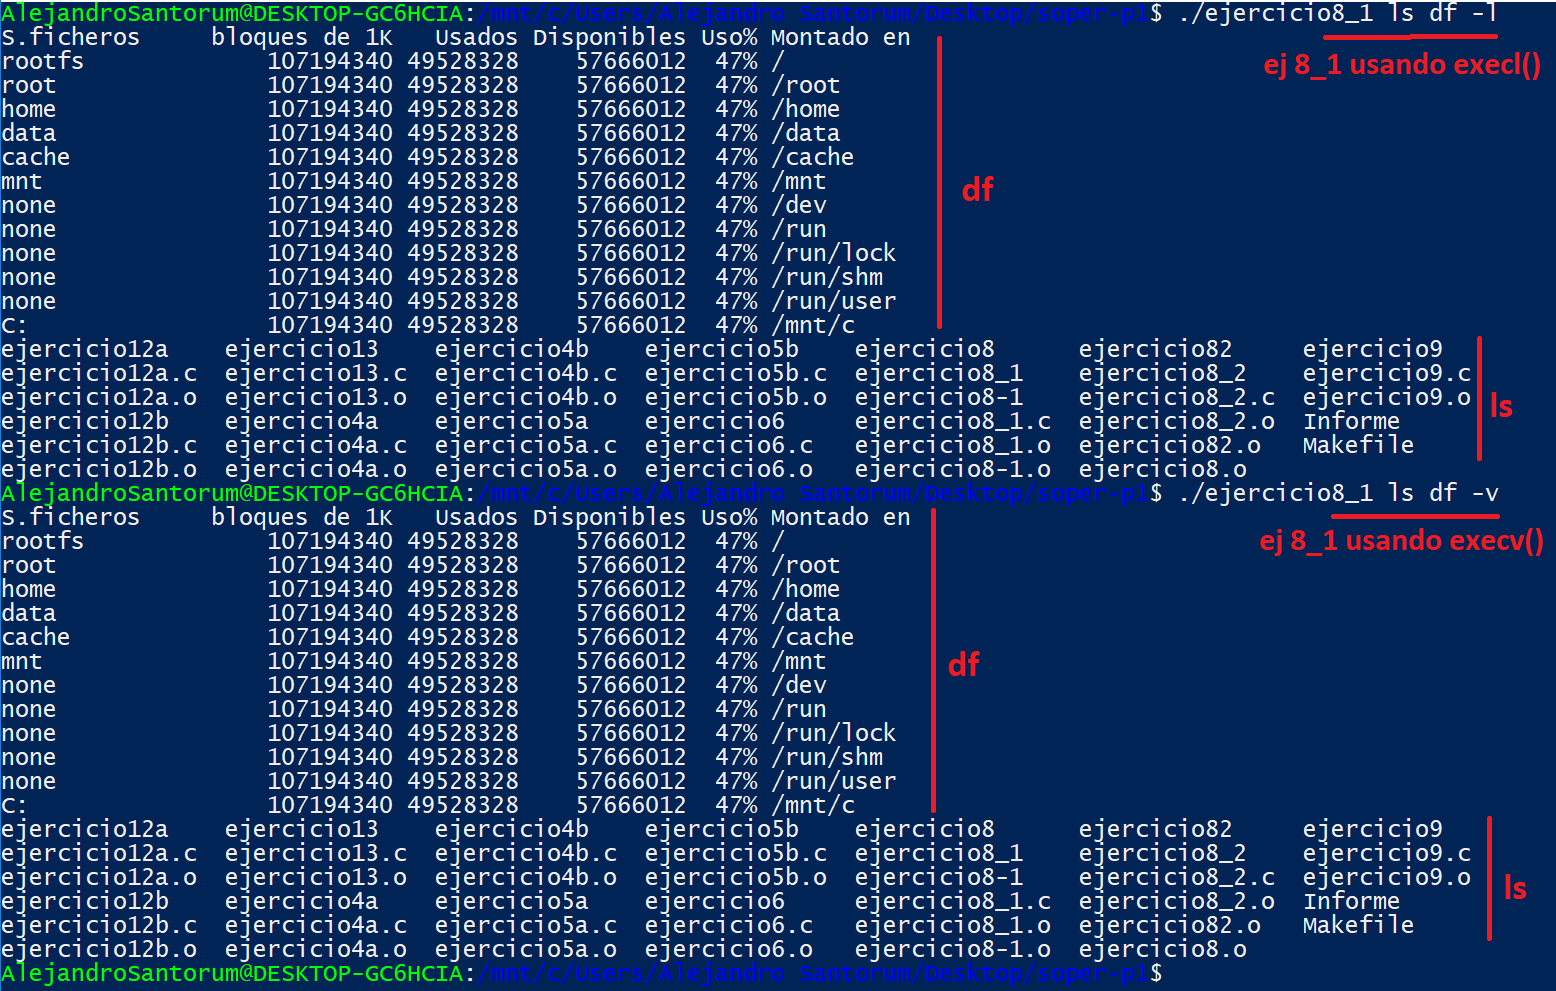
\includegraphics[scale=0.8]{ej8_1.PNG}
\end{center}
\begin{center}
	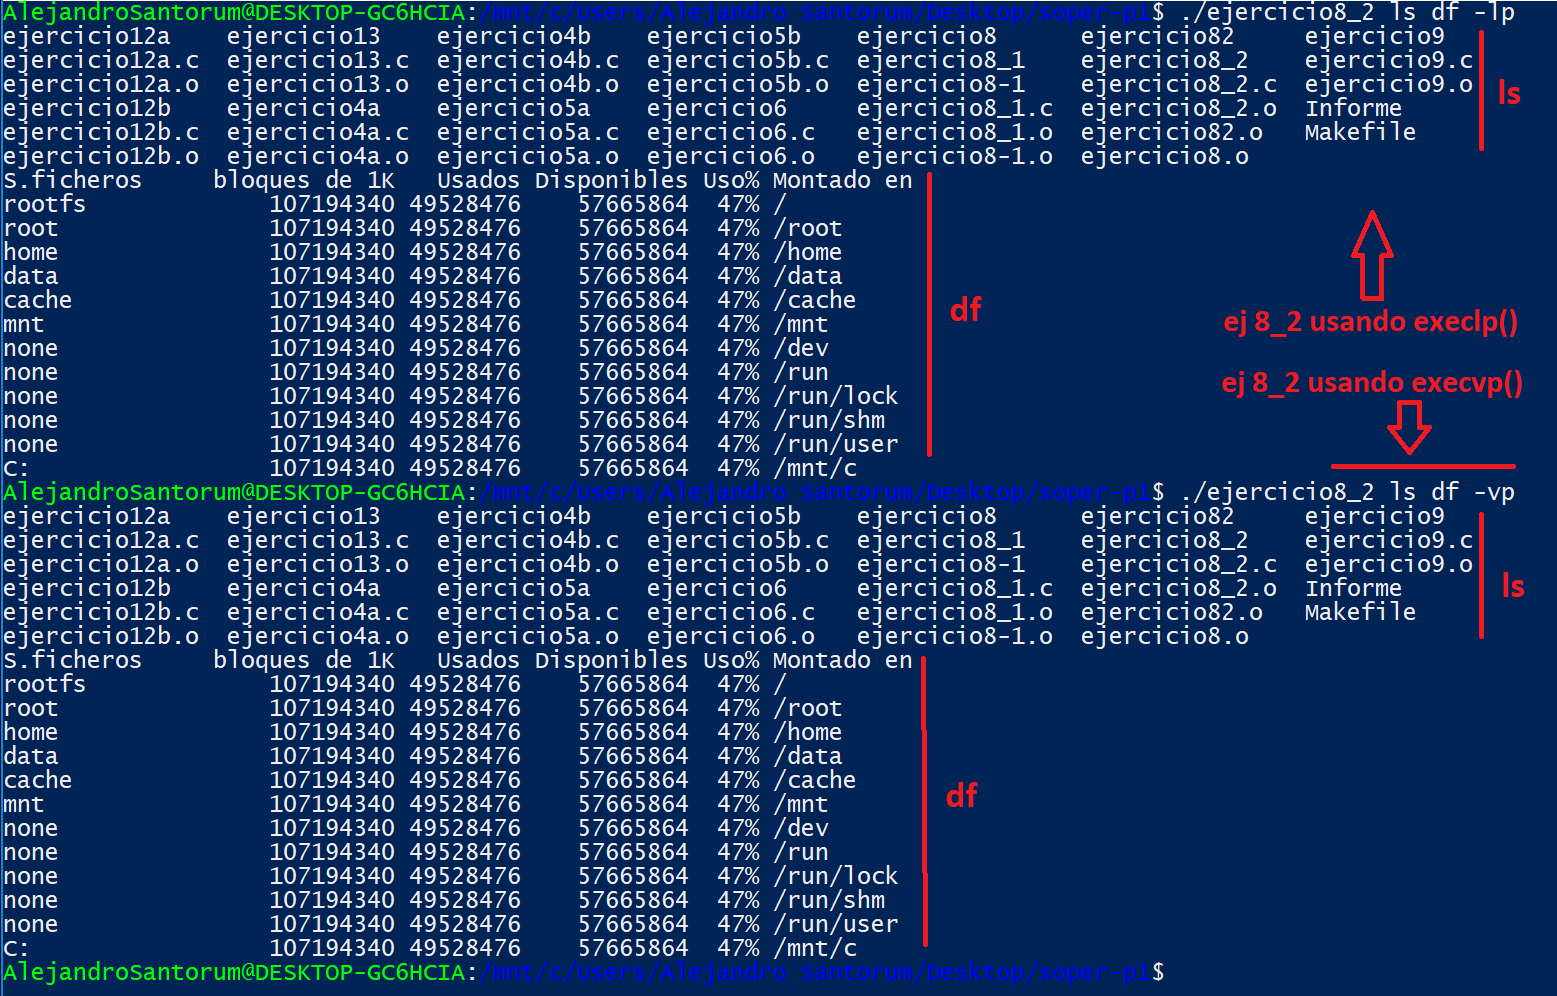
\includegraphics[scale=0.8]{ej8_2.PNG}
\end{center}



\section{Ejercicio 9}
Si hemos dicho que el ejercicio anterior era completo y enriquecedor, este no se queda atrás.\\ Consiste en aprender como comunicar dos o más procesos entre si con la ayuda de las tuberías o pipes.\\\\
El problema pedía que se crearan cuatro procesos hijos que, con los operandos adquiridos en el proceso padre y pasados a sus hijos por tuberías, realizasen cada uno de ellos diferentes operaciones y devolviesen al proceso padre el resultado mediante otras tuberías.\\\\
Vamos a explicar el programa. Lo primero que llama la atención es la declaración fd[2*N\_CHILDS][2]. Lo que se está haciendo es preparar 16 enteros que serán nuestras futuras tuberías, que se crearán con la función \texttt{pipe(fd[h])}. ¿Por qué se necesitan 16? Pues bien, cada hijo tiene que comunicarse con su padre. En primer lugar, es el padre que envía (escribe) a cada hijo (lee) los operandos a utilizar, por lo que tendrán que cerrar los extremos de las tuberías correspondientes, el padre cierra lectura y el hijo escritura.\\Una vez se hayan hecho las operaciones, los procesos cambian los papeles, los hijos envían el resultado (escriben) al proceso padre (lee), por lo que los hijos tendrán que cerrar el extremo de lectura y el padre el de escritura. A lo largo de este proceso se han necesita 4 tuberías por cada par padre-hijo, como tenemos 4 hijos (4 operaciones a realizar) resulta en un total de 16 tuberías.\\\\
Después de lo descrito anteriormente, no queda mucho que explicar. Simplemente contar que se utilizan las funciones de bajo nivel para control de ficheros \texttt{read()} y \texttt{write()}, pues las tuberías son en realidad ficheros de uso compartido por el proceso padre y su proceso hijo.\\\\
Es importante hacer una observación y es que hay que tener cuidado con el overflow que podría ocasionar la introducción de operandos grandes, ya que el factorial crece bastante rápido. El factorial de 20 ya es igual a 2432902008176640000. Se han utilizado variables de tipo long long para hacer el cálculo, pero ya vemos que con un operando grande el cálculo con factoriales y/o potencias desborda enseguida. 
De seguido, mostramos tres ejecuciones del programa con operandos diferentes.
\begin{center}
	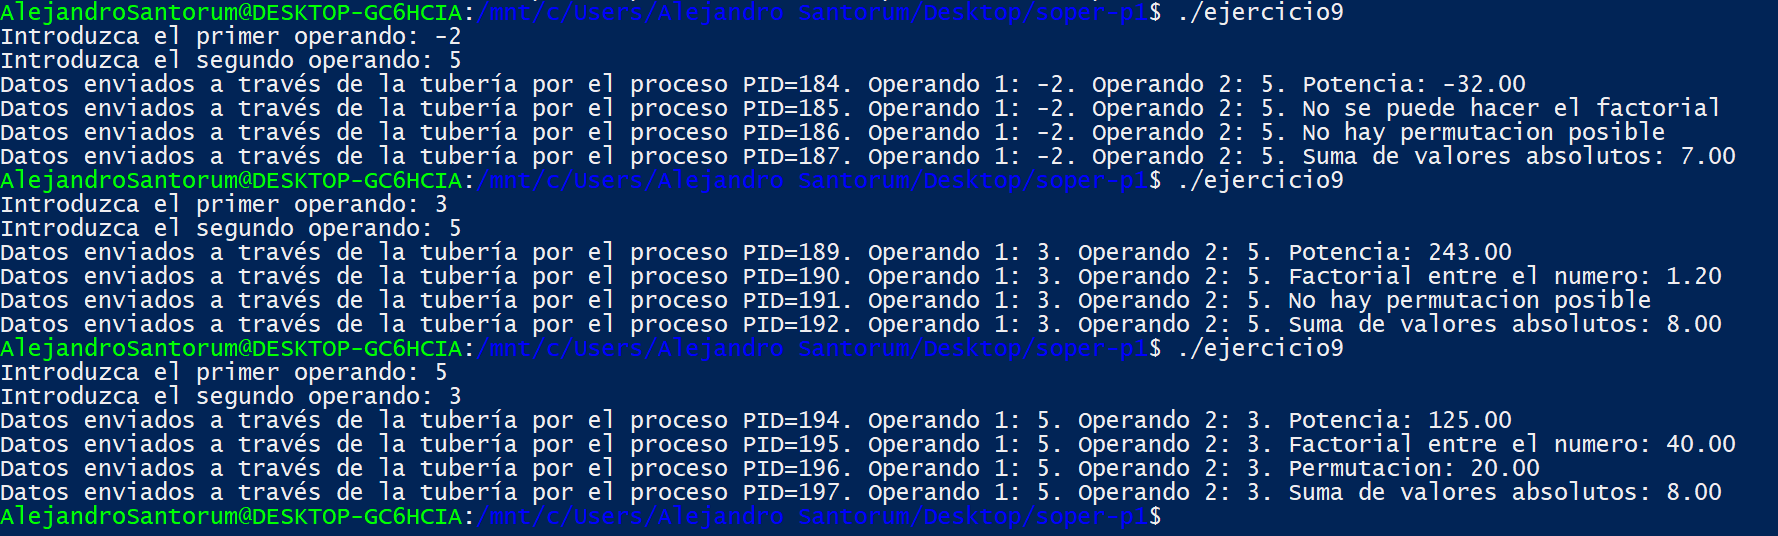
\includegraphics[scale=0.75]{ej9.PNG}
\end{center}
Podemos observar que las operaciones son las correctas, siempre y cuando se puedan realizar. Se ejemplifica esto último en las ejecuciones número 1 y número 2.\\ En la primera no se ha podido calcular el factorial porque uno de los números es negativo (pasaría lo mismo si 02 fuera menor que cero), ni tampoco las permutaciones por el mismo motivo.\\ En la segunda sí que se ha podido calcular el factorial, pero no las permutaciones porque el operando número 1 era mayor que el número 2.\\ En la ejecución número 3 no hay errores con los operandos, por lo que las operaciones son realizadas correctamente.


\section{Ejercicio 12}
Este ejercicio se divide en dos programas (ejercicio12a y ejercicio12b), que hacen la misma función: calcular los N primeros primos. En el primero se calculan los N primeros primos en 100 procesos diferentes simultáneamente y en el segundo, lo mismo, pero esta vez utilizando 100 hilos.\\\\
Este ejercicio se enfoca en calcular el tiempo de ambos programas y compararlos, contrastando el resultado obtenido con la teoría.\\\\
En el ejercicio 12a se realizará el cálculo de los 10000 primeros primos en 100 procesos hijos y se medirá lo que ha tardado para posteriormente, en el ejercicio que precede a este, el ejercicio 12b, compararlo con el tiempo que han necesitado 100 hilos diferentes en calcular también los 10000 primeros primos.\\\\
Analizamos ahora el programa 12a. Comenzamos creando 100 procesos hijos de un único padre, el proceso que lanza el programa. Todos los hijos realizan el cálculo de los 10000 primeros, y el padre los esperará a todos. Se calcula el tiempo entre antes de llamar a los procesos hijos y después de esperarlos a todos para luego mostrarlo por pantalla.\\\\
Comentemos ahora un poco el programa 12b. Para empezar, la función que crea los hilos es \texttt{pthread\_create(...)}, que es lo análogo con los procesos a \texttt{fork()}. Del mismo modo, \texttt{pthread\_join(...)} cumple la misión de \texttt{wait()}.\\ El constructor de hilos tiene como argumetos la dirección de un hilo o pthread\_t, de segundo los atributos de la creación del hilos, que si es NULL se escogerán por defecto. De tercero el nombre de la función que será llamada automáticamente en el hilo y, por último, el argumento void* que recibe el parámetro de entrada de la función que va a ser llamada. Una técnica muy usada es pasar todos los argumentos que se quieran mediante una estructura "casteada" a void*.\\\\
Mostremos la salida que origina este programa y el anterior para comparar los tiempos de ejecución.
\begin{center}
	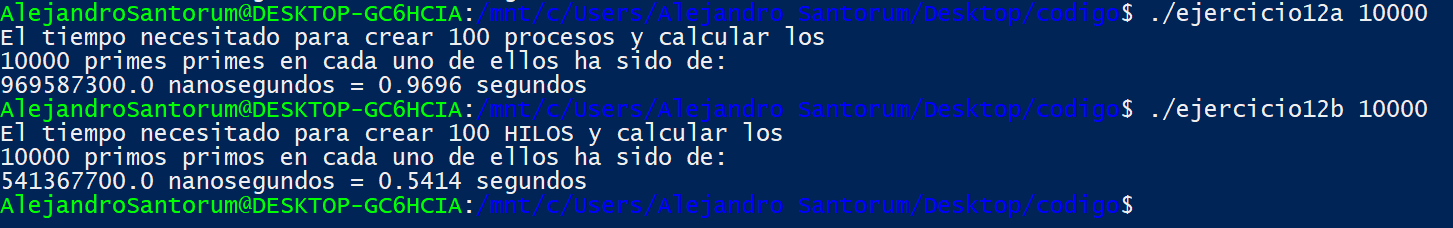
\includegraphics[scale=0.9]{ej12aY12b.PNG}
\end{center}
En este ejemplo en particular, el tiempo utilizando procesos ha sido de 0.97 segundos y el mismo programa utilizando hilos ha sido de 0.54 segundos.\\ El tiempo utilizando hilos ha sido prácticamente la mitad, como cabía de esperar, pues es mucho más eficiente la creación, comunicación y eliminación de hilos que de procesos.\\\\ Esto es debido a que la creación de los hilos es mucho más eficiente que la de los procesos, ya que necesitan copiar muy poca memoria, solo la pila del propio hilo, a diferencia de los procesos, que tenían que duplicar toda la memoria reservada/utilizada.\\Por otro lado, es mucho más rápido cambiar los estados de Listo-Ejecución entre hilos que entre procesos.\\Por último, la comunicación de hilos es mucho más rápida que la de los procesos, ya que comparten la memoria común del proceso. 



\section{Ejercicio 13}
Llegamos al último ejercicio de la práctica 1. Esta vez se nos pide calcular el producto de dos escalares por dos matrices en dos hilos trabajando en paralelo.\\ La secuencia del programa es pedir la dimesión de las matrices al usuario, para después preguntarle por los dos escalares y las dos matrices. Después de esto, dos hilos paralelos calcularán el producto de un escalar por una matriz cuadrada cada uno, mostrando las operaciones cada vez que acaban con una fila.\\\\
Se puede resumir la estrategia seguida muy fácilmente. Se ha programado una función que será ejecutada por dos hilos al mismo tiempo, cuya única misión es imprimir las matrices pasadas por el argumento void* que apunta a una estructura con todos los datos que necesita.\\ En el programa principal, main, simplemente se piden los datos al usuario y se guardan en los campos de la estructura. Pthread\_create(...) hace el resto.\\
Comentar que se ha hecho el apartado final, en el que cada hilo puede conocer por donde va el otro. Mostramos ahora un ejemplo de su ejecución.
\begin{center}
	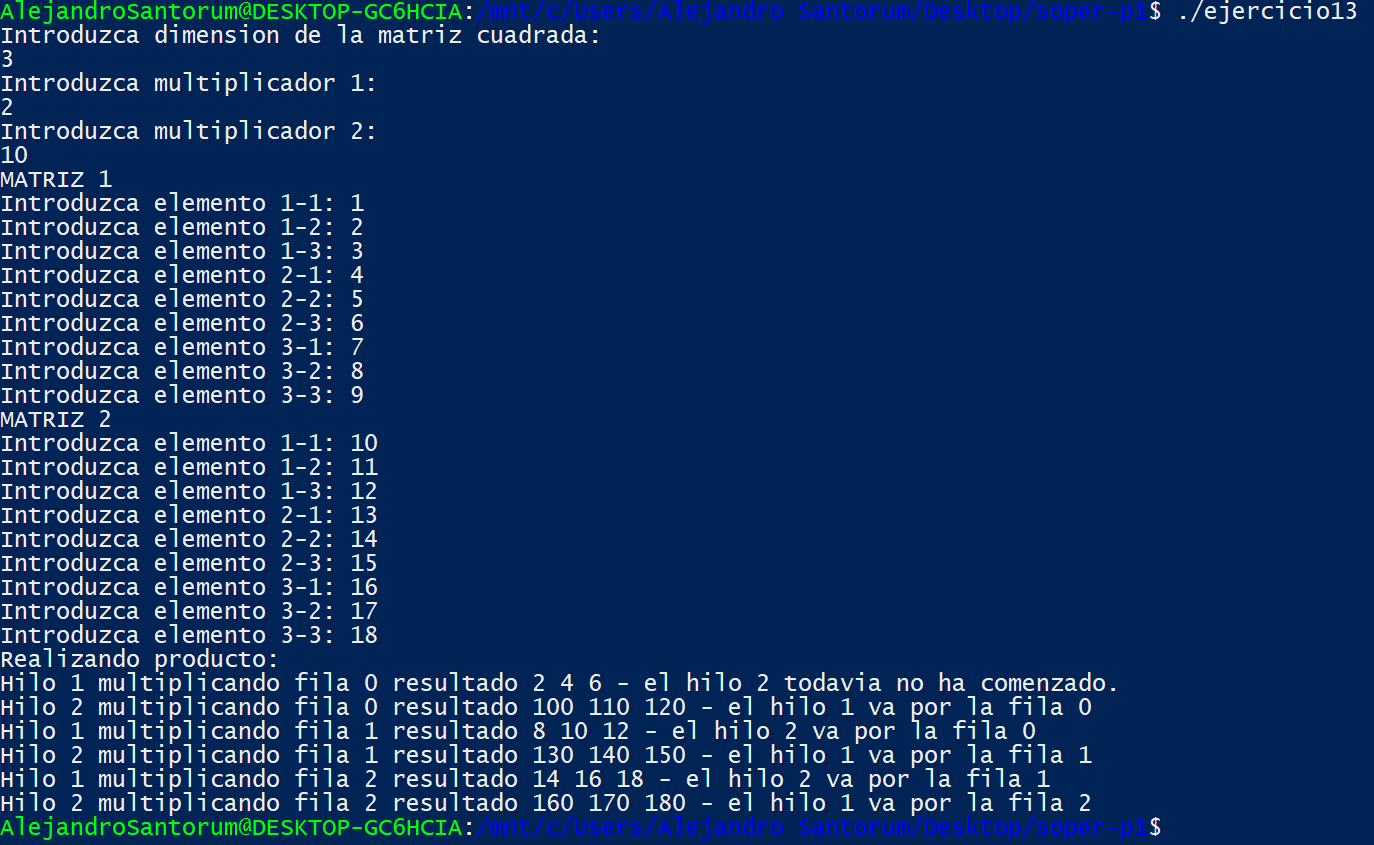
\includegraphics[scale=0.93]{ej13.PNG}
\end{center}
Antes que nada comentar una decisión de diseño: en la documentación de la práctica se ejemplificaba la introducción de las matrices tal que así:
\begin{center}
	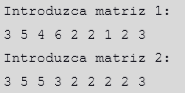
\includegraphics[scale=2]{intr_matriz_doc.PNG}
\end{center}
A diferencia de nuestra forma, que pedimos elemento a elemento. Esto puede ser un poco más incómodo para quien utiliza la línea de comandos, pero mejora la eficiencia del programa al evitar tener que "tokenizar" la string que sería obtenida por el método del ejemplo de la documentación., pasando de un coste $O(n)$ siendo $n = dim^2$ a un coste $O(1)$ ya que el dato es introducido directamente en la matriz.\\\\ Dejando ya a parte el estilo de código, comentar la estrategia seguida para comunicar un hilo con otro. Hemos utilizado el hecho de que los hilos no duplican la memoria reservada como sí hacen los procesos para poder comunicarlos mediante dos punteros de tipo char*. Uno de ellos es destinado a la escritura del hilo 1 y lectura del hilo 2, y el otro a la lectura del hilo 1 y escritura del 2.\\ Mediante este método, podemos pasar información de por qué parte del cálculo del producto se encuentran e imprimirlo por pantalla, tal y como se muestra en la imagen.



\section{Conclusión y comentarios finales}
Ha sido una práctica larga y productiva, en la que hemos aprendido muchas cosas sobre la programación orientada a la multi-tarea mediante los procesos e hilos.\\\\
Los primeros ejercicios han tenido el objetivo de enseñar cómo funciona el fork() y las interaciones proceso padre-proceso hijo.\\ Después se ha enfocado más a la intercomunicación de procesos para poder intercambiarse información y/o datos.\\ Por último, hemos obtenido la intuición de qué es un hilo y sus diferencias (para bien o para mal) con los procesos.
\end{document}